%!TEX TS-program = xelatex 
%!TEX encoding = UTF-8 Unicode 

\documentclass[fontsize=11pt, paper=a4, 
DIV15,
headings=normal,
parskip=half-, 
numbers=noenddot]{scrartcl}

\usepackage[british]{babel} 

\usepackage{fontspec,xltxtra,xunicode} 
\defaultfontfeatures{Mapping=tex-text} 

\setromanfont[Mapping=tex-text]{DejaVu Serif}
\setsansfont[Scale=MatchLowercase,Mapping=tex-text]{Helvetica} 
\setmonofont[Scale=1.0]{Courier New} 

\frenchspacing

\usepackage{graphicx}
\graphicspath{{../../bilder/chinese/}}

\usepackage{longtable}

%%%

\input{../../abbreviations/abbreviations_2}

\newcommand{\hash}{{\char"0023}}
\newenvironment{typeChinese}{\begin{alltt}\s\begin{tabular}{@{}l}}{\end{tabular}\end{alltt}}

\newcommand{\chin}[1]{{\fontspec{Sun-ExtA}{#1}}}
\newcommand{\sunExtA}[1]{{\fontspec{Sun-ExtA}{#1}}}
\newcommand{\sunExtB}[1]{{\fontspec{Sun-ExtB}{#1}}}
\newcommand{\extB}[1]{{\fontspec{Sun-ExtB}{#1}}}

\newcommand{\mincho}[1]{{\fontspec{MS Mincho}{#1}}}
\newcommand{\hira}[1]{{\fontspec{HiraMinPro-W3}{#1}}}

% Verkürzung von \bold und \chin:
% schon vorhanden: ch, c, s;  b, bf
% noch nicht vorhanden: sun (bringt aber nicht viel)
\newcommand{\f}[1]{\bold{#1}} % f für fett
\newcommand{\z}[1]{\chin{#1}} % z für Zeichen

%%%

\begin{document}

\begin{center}
{\fontspec{Helvetica}{\LARGE \textbf{
Data Entry Specs for Chinese Text }}} \\[5mm]
\large Wolfgang Schmidle, Martina Siebert, \\[1mm] 
Martin Hofmann, Klaus Thoden, Malcolm D. Hyman

\normalsize Max Planck Institute for the History of Science, Berlin, Germany

Version 2.1 \\[1mm]
\today
\end{center}

\tableofcontents

\newpage

\section{File Conventions}
\label{section file conventions}

\begin{mainrule}
Save the text in plain text format (§.txt§) with Unicode §utf-8§ encoding. If the text is saved in more than one file, number the parts, for example §Euclid_part_001.txt§, §Euclid_part_002.txt§, and so on. Create a §zip§ archive of all files.
\end{mainrule}

\begin{mainrule}
Make use of the complete character repertoire found in Unicode version 5.1.
\end{mainrule}

\begin{clarification}
This includes characters in the following Unicode blocks when applicable: 

\begin{itemize}
\item CJK Unified Ideographs Extension A (U+3400 -- U+4DFF)
\item CJK Unified Ideographs Extension B (U+20000 -- U+2A6DF)
%\item CJK Compatibility Ideographs Supplement (U+2F800 -- U+2FA1F)
\end{itemize}
At this point, do not make use of the characters in Extension C or D.
\end{clarification}

\begin{mainrule}
We will also need the list of unknown characters (see \sect{section unknown characters}) and the list of character variants (see \sect{section character variants}). Please send each list in two versions, namely in the original file format (e.g. RTF, DOC, XLS) and as PDF. If the lists are handwritten, scan them and save them as PDF files. 
\end{mainrule}


\section{General Markup}

\begin{mainrule}
Type the entire contents of one page, then go on to the next page. Do not mix the contents of different pages.
\end{mainrule}

\tocspace
\subsection{Page Breaks, Page Numbers and Running Heads}

\label{section page breaks}

\begin{mainrule}
Page breaks are marked by §<pb>§. If the page has a page number, type it within the §<pb>§ tag, e.g. §<pb §\z{六}§>§. Type the page number exactly as it appears in the book. If there is a running head on the page, it is marked by §<rh>§ and §</rh>§. Type the running head immediately after the §<pb>§ tag. 
\end{mainrule}

\begin{clarification}
Type the §<pb>§ and §<rh>§ tags before you type any page content. 
\end{clarification}

\begin{mainrule}
The centre section of a traditional printing page (\emph{banxin} \z{版心}) is equivalent to a running head in a western book layout. In this case, repeat §<pb>§ and the running head for each half-page, but add §a§ and §b§ to the page number, e.g. §<pb §\z{三}§a>§ and §<pb §\z{三}§b>§, or §<pb a>§ and §<pb b>§ if there is no page number.
\end{mainrule}

\begin{clarification}
If the characters of the running head are cut off on the scanned page, type them anyway. Type large spaces in the running head as a single IDEOGRAPHIC SPACE character U+3000.
\end{clarification}

\begin{note}
In the digitization of the book, the two half-pages may be on the same scan or on two consecutive scans.
\end{note}

\begin{tabular}{@{}ll}
\parbox[b]{116mm}{
\htsc{Examples} \\[18mm]
\begin{typeChinese}
\f{<pb} \z{三十二}\f{a><rh>}\z{泰西事物}\f{<}\z{起}\f{V>}\z{原 第十一章}\f{</rh>} \\
\\
\f{<pb} \z{十二}\f{a><rh>}\z{事物攷辨卷之六十三 }\f{<sm>}\z{植物}\f{</sm>}\z{ 帶經堂}\f{</rh>} \\
\\ 
\f{<pb} \z{一}\f{a><rh>}\z{閩產}\f{<}\z{錄}\f{V>}\z{異 卷一}\f{<sm>}\z{穀屬}\f{</sm></rh>} \\
\\ 
\f{<pb} \z{一}\f{b><rh>}\z{閩產錄異 卷一}\f{<sm>}\z{穀屬}\f{</sm></rh>} \\[18mm]
\end{typeChinese}} 
&
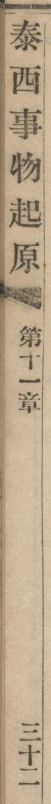
\includegraphics[height=8cm]{chinese_rh_1} \qquad
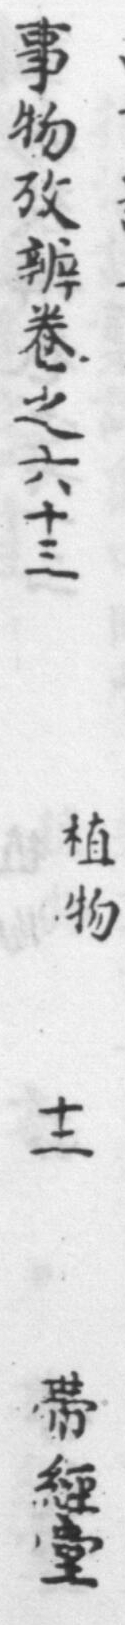
\includegraphics[height=8cm]{chinese_rh_2} \qquad
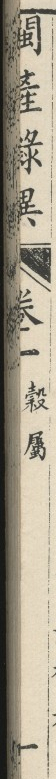
\includegraphics[height=8cm]{chinese_rh_3a} \qquad
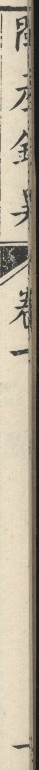
\includegraphics[height=8cm]{chinese_rh_3b}
\end{tabular}

\vspace{3mm}
\begin{crossref}
For §<sm>§ see \sect{section chinese small characters}. An example of two complete half-pages with their running heads can be seen in \sect{section chinese paragraphs}.
\end{crossref}

\begin{note}
For §< V>§ (i.e. marking character variants which are not included in Unicode 5.1) see \sect{section character variants}. 
\end{note}


\tocspace
\subsection{Text Blocks}

\begin{mainrule}
Type a return after each line of the printed page.
\end{mainrule}

\begin{clarification}
Do not insert a space at the end of the line. 
\end{clarification}



\subsubsection{Headings}
\label{section chinese headings}

\begin{mainrule}
Headings are marked by §<h> </h>§. If you can identify a heading as the book title, use §<ti>§ for the whole line. If you can identify a heading as the name of the author, compilator, proofreader etc. (\emph{ti} \z{題}), use §<ti>§ too. If a text has different levels of headings, use §<h 1>§ for all headings on the highest level, §<h 2>§ for all headings on the second highest level, and so on.
\end{mainrule}

\begin{clarification}
If a heading, book title, author, etc. is indented, do not mark this. Type large spaces in the heading as a single IDEOGRAPHIC SPACE character U+3000.
\end{clarification}

%\begin{note}
%Typically, a book has at most three different heading levels, i.e. §<h 1>§,  §<h 2>§ and  §<h 3>§. 
%\end{note}


%\begin{example} % Text 17-1, p.11; Text 14, p.74

\begin{tabular}{@{}ll}
\parbox[b]{131mm}{
\htsc{Example} \\[3mm]
\begin{typeChinese}
\f{<ti>}\z{閩產}\f{<}\z{錄}\f{V>}\z{異卷一}\f{</ti>} \\
\f{<stamp>} \\
\f{<ti>}\z{侯官郭柏}\f{<}\z{蒼}\f{R><}\z{蒹}\f{R>}\z{秋輯}\f{</ti>} \\
\f{<h 1>}\z{穀屬}\f{</h>} \\
\f{<h 2>}\z{早占城晚占城}\f{</h>}\z{ }\f{<p>}\z{有赤白二種宋真宗以福建田多高} \\
\z{仰聞占城稻耐旱遣使求其種得二十石以遺閩農} \\
\z{今延建邵福甯龍巖種者尚少餘則徧種矣各郡}\f{<}\z{縣}\f{V>} \\
... \f{</p>} \\
\f{<h 2>} ... \f{</h>}\z{ }\f{<p>} ... \\
... \f{</p>} \\[20mm]
\end{typeChinese}
} & 
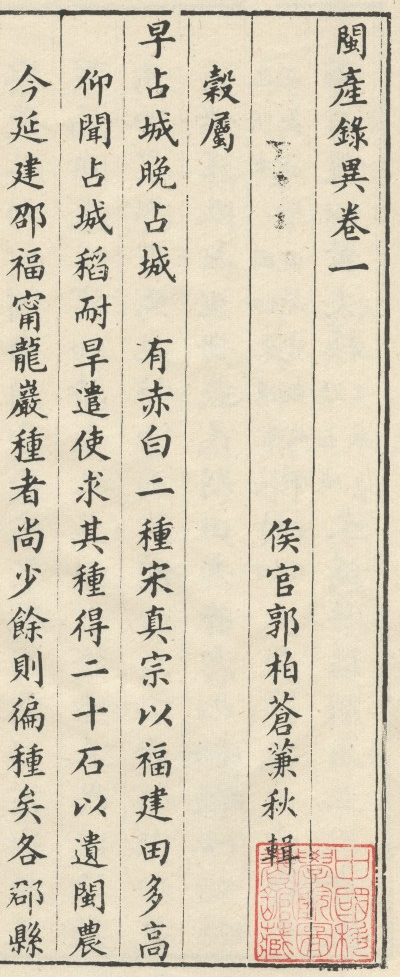
\includegraphics[height=8cm]{text17-1p11}
\end{tabular}

\vspace{-8mm}
\begin{crossref}
For §<stamp>§ see \sect{section chinese stamps}. For §<p>§ see \sect{section chinese paragraphs}. 
\end{crossref}

\vspace{5mm}
\begin{note}
In the transcription of this example, there are three headings on two different levels (§<h 1>§, §<h 2>§, §<h 2>§). In the example in \sect{section chinese paragraphs} there are two headings, both on level 2 (§<h 2>§, §<h 2>§). §<h 1>§ appears on other pages of the book.
\end{note}

%\begin{note}
%In this example, the base line for indentation (see \sect{section chinese paragraphs}) would be one character below the printing frame.
%\end{note}

%(We do not make them mark “Sperrung” in book titles.)


\subsubsection{Paragraphs}
\label{section chinese paragraphs}

\begin{mainrule}
Paragraphs are marked by §<p>§ and §</p>§. Indented paragraphs are marked by one or more §i§, e.g. §<p iii>§ for a paragraph that is indented by three character spaces. Outdented paragraphs are marked by one or more §x§, e.g. §<p x>§.
\end{mainrule}

\begin{clarification}
Every part of the book has a base line where all unindented paragraphs start. The base lines in the preface or table of contents may be different from the base line in the main text. Mark indentations relative to the base line. The indentation symbols §i§ and §x§ always refer to the first line of the paragraph. The remaining lines of the paragraph may have the same or a different indentation, which is not marked. If a paragraph is preceded by a sub-heading in the same line, as in the example in \sect{section chinese headings}, do not mark the indentation at all. 
\end{clarification}

\begin{clarification}
Make sure that for each §<p>§ there is a corresponding §</p>§ somewhere. If a paragraph starts and ends on different pages, the §<p>§ and §</p>§ tags are on these different pages.
\end{clarification}

\begin{tabular}{@{}ll}
\parbox[b]{29.5mm}{
\htsc{Example} \\[80mm]
} & 
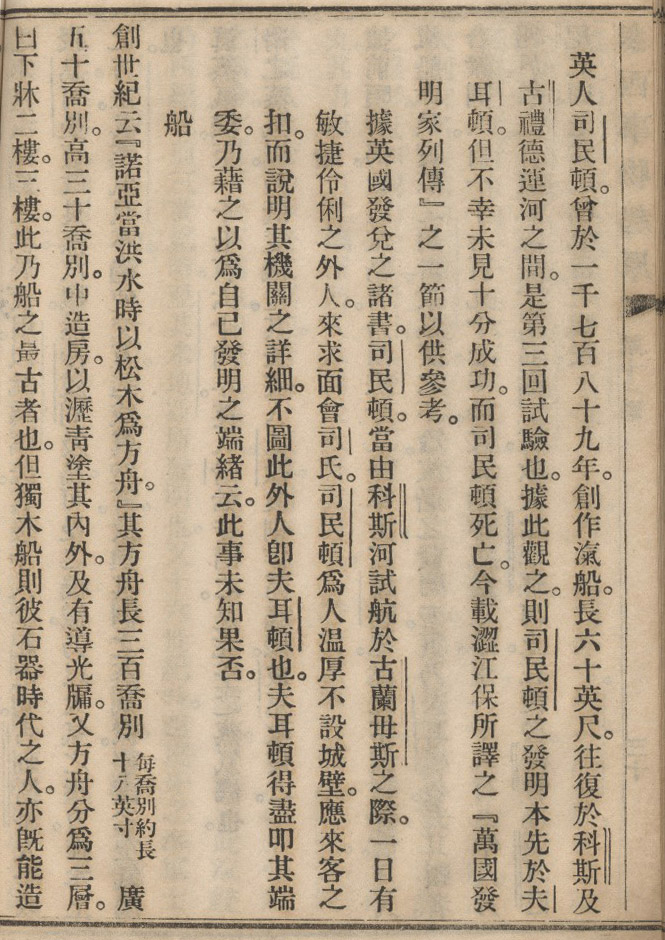
\includegraphics[height=9cm]{text14p74_neu} \quad
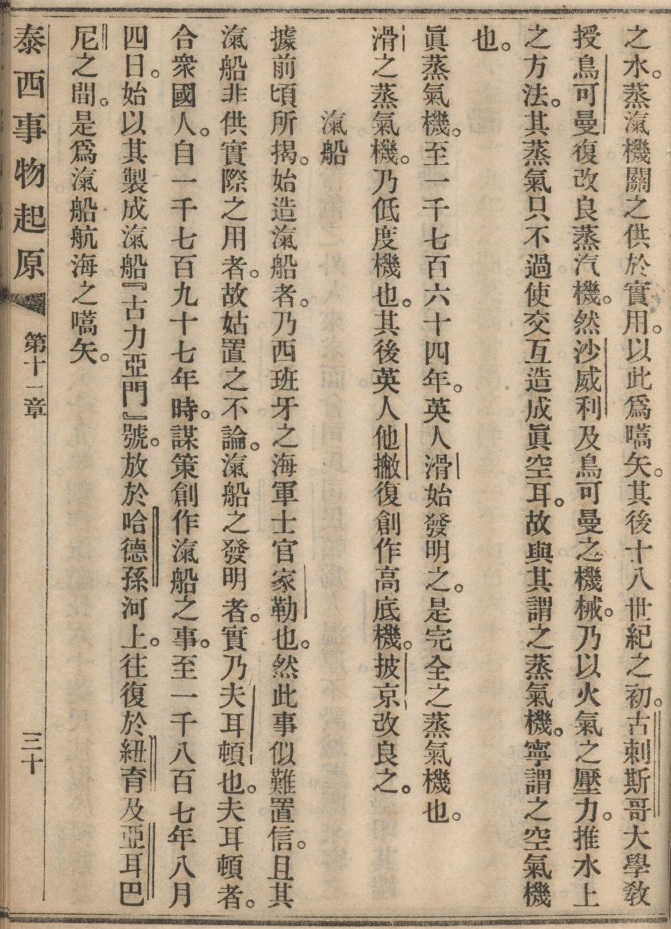
\includegraphics[height=9cm]{text14p73}
\end{tabular}

\begin{typeChinese}
\f{<pb} \z{三十}\f{a><rh>}\z{泰西事物}\f{<}\z{起}\f{V>}\z{原 }\f{<sm>}\z{第十一章}\f{</sm></rh>} \\
\z{之水。蒸滊機關之供於實用。以此爲嚆矢。其後十八世}\f{<}\z{紀}\f{R>}\z{之初。}\f{<dl>}\z{古剌斯哥}\f{</dl>}\z{大學教} \\ 
\z{授}\f{<sl>}\z{鳥可曼}\f{</sl>}\z{復改良蒸汽機。然}\f{<sl>}\z{沙威利}\f{</sl>}\z{及鳥可曼之機械。乃以火氣之壓力。推水上} \\
\z{之方法。其蒸氣只不}\f{<}\z{過}\f{RV>}\z{使交互造成眞空耳。故與其謂之蒸氣機。寧謂之空氣機} \\
\z{也。}\f{</p>} \\
\f{<p>}\z{眞蒸氣機。至一千七百六十四年。英人}\f{<sl><}\z{滑}\f{V></sl>}\z{始發明之。是完全之蒸氣機也。} \\
\f{<sl>}\z{滑}\f{</sl>}\z{之蒸氣機。乃低度機也。其後英人}\f{<sl>}\z{他撇}\f{</sl>}\z{復創作高底機。}\f{<sl>}\z{披京}\f{</sl>}\z{改良之。}\f{</p>} \\
\f{<h 2>}\z{滊船}\f{</h>} \\
\f{<p>}\z{據前頃所揭。始造滊船者。乃西班牙之海軍士官}\f{<sl>}\z{家勒}\f{</sl>}\z{也。然此事似難}\f{<}\z{置}\f{V>}\z{信。且其} \\
\z{滊船非供實際之用者。故姑置之不論。滊船之發明者。實乃}\f{<sl>}\z{夫耳頓}\f{</sl>}\z{也。夫耳頓者。} \\
\z{合衆國人。自一千七百九十七年時。謀策創作滊船之事。至一千八百七年八月} \\
\z{四日。始以其製成滊船『古力亞門』號。放於}\f{<dl>}\z{哈德孫}\f{</dl>}\z{河上。往復於}\f{<dl>}\z{紐育}\f{</dl>}\z{及}\f{<dl>}\z{亞耳巴} \\
\z{尼}\f{</dl>}\z{之間。是爲滊船航海之嚆矢。}\f{</p>} \\
\\
\f{<pb} \z{三十}\f{b><rh>}\z{泰西事物起原 }\f{<sm>}\z{第十一章}\f{</sm></rh>} \\
\f{<p i>}\z{英人}\f{<sl>}\z{司民}\f{</sl>}\z{頓。曾於一千七百八十九年。創作滊船。長六十英尺。往復於}\f{<dl>}\z{科斯}\f{</dl>}\z{及} \\
\f{<dl>}\z{古禮}\f{</dl>}\z{德運河之間。是第三回試驗也。據此觀之。則}\f{<sl>}\z{司民頓}\f{</sl>}\z{之發明本先於}\f{<sl>}\z{夫} \\
\z{耳}\f{</sl>}\z{頓。但不幸未見十分成功。而司民頓死亡。今載澀江保所譯之『萬國發} \\
\z{明家列傳』之一節以供參考。}\f{</p>} \\
\f{<p iii>}\z{據英國發兌之諸書。}\f{<sl>}\z{司民}\f{</sl>}\z{頓。當由}\f{<dl>}\z{科斯}\f{</dl>}\z{河試航於}\f{<sl>}\z{古蘭毋斯}\f{</sl>}\z{之際。一日有} \\
\z{敏捷}\f{<}\z{伶}\f{V>}\z{俐之外人。來求面會}\f{<sl>}\z{司}\f{</sl>}\z{氏。}\f{<sl>}\z{司民頓}\f{</sl>}\z{爲人温厚不設城壁。應來客之} \\
\z{扣。而說明其機關之詳細。不圖此外人卽夫}\f{<sl>}\z{耳頓}\f{</sl>}\z{也。夫耳頓得盡叩其端} \\
\z{委。乃藉之以爲自己發明之端}\f{<}\z{緖}\f{R>}\z{云。此事未知果否。}\f{</p>} \\
\f{<h 2>}\z{船}\f{</h>} \\
\f{<p>}\z{創世紀云『諾亞當洪水時以松木爲方舟』。其方舟長三百喬別}\f{<sm>}\z{每喬別}\f{<}\z{約}\f{V>}\z{長}\f{\bs\bs}\z{十八英寸}\f{<sm>}\z{ }\f{<}\z{廣}\f{V>} \\
\z{五十喬別。高三十喬別。中造房。以瀝靑塗其內外。及有導光牖。又方舟分爲三層。} \\
\z{曰下牀二樓。三樓。此乃船之最古者也。但獨木船則彼石器時代之人。亦}\sunExtA{既}\z{能造} \\
\end{typeChinese}

%\vspace{-2mm}
\begin{crossref}
For §<sm>§ see \sect{section chinese small characters}. For §<sl>§ and §<dl>§ see \sect{section chinese underlinings}.
\end{crossref}

\vspace{3mm}
\begin{note}
For the marking of character variants (§< V>§, §< R>§, §< RV>§) see \sect{section character variants}. Only the first appearance of each character variant is marked. For instance, \z{起} is marked in the first running head but not in the second one. 
% The two half-pages are treated as if they were the beginning of the text. Consequently, \z{起} is marked even though it already appears on earlier pages.
(In addition, every example in the Data Entry Specs is treated as if it was the beginning of a text, i.e. \z{起} is marked on the first half-page even though it already appears on earlier pages of the text.)
\end{note}


\tocspace
\subsection{Structured Text}
\label{section structured text}

\subsubsection{Tables}
\label{section tables}

\begin{mainrule}
A table is marked by §<tb>§ and §</tb>§. Use §#§ as field separators. Type a return after each row. Do not type horizontal or vertical lines. 
\end{mainrule}

\begin{clarification}
Type the §<tb>§ and §</tb>§ tags on separate lines. Do not mark indentations. The field separators may be lines or large spaces.
\end{clarification}

\begin{clarification}
If you can identify a single space within a name etc. as a decorative space to make the table layout optically more pleasing, do not type it.
\end{clarification}

\vspace{3mm}
\begin{tabular}{@{}ll}
\parbox[b]{88mm}{
\htsc{Example} \\
\begin{typeChinese}
\f{<p>}\z{今日諸國所用文字之數如左}\f{</p>} \\
\f{<tb>} \\
\z{英吉利} \f{\hash} \z{二十六} \\
\z{法蘭西} \f{\hash} \z{二十三} \\
\z{西班牙} \f{\hash} \z{二十七} \\
\z{希臘} \f{\hash} \z{二十四} \\
\z{斯格拉}\f{<}\z{窩}\f{V>}\z{尼亞} \f{\hash} \z{二十七} \\
\z{德意志} \f{\hash} \z{二十六} \\
\z{意大利} \f{\hash} \z{二十} \\
\z{俄}\f{<}\z{羅}\f{V>}\z{斯} \f{\hash} \z{四十一} \\
\z{拉丁} \f{\hash} \z{二十三} \\
\z{希伯流} \f{\hash} \z{二十二} \\
\z{梵字} \f{\hash} \z{五十} \\
\f{</tb>} 
\end{typeChinese}
} &
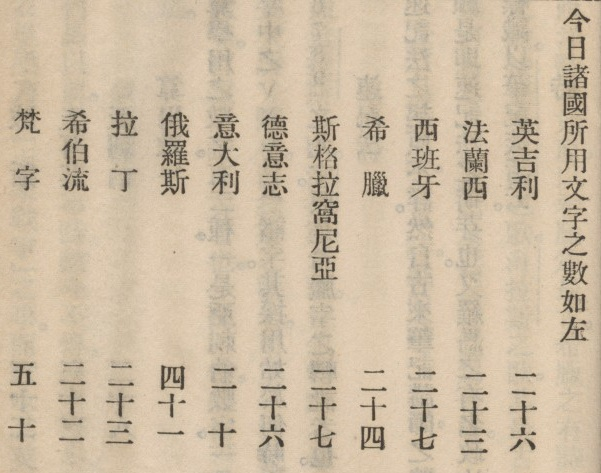
\includegraphics[height=6cm]{text14p43} 
\end{tabular}


\subsubsection{Lists}
\label{section chinese lists}

%\mehrzeilen[5]

\begin{mainrule}
A list is marked by §<list>§ and §</list>§. Use §#§ for large spaces, if there are any.
\end{mainrule}

\begin{clarification}
Type the §<list>§ and §</list>§ tags on separate lines. If the items on consecutive text lines belong to the same list entry, use §#§ at the beginning of the next line. Do not mark indentations. 
\end{clarification}

\begin{clarification}
Unlike in tables, type each single space, i.e. do not omit single spaces even if they seem to be merely decorative.
\end{clarification}

\begin{tabular}{@{}ll}
\parbox[b]{112mm}{
\htsc{Example} \\
\begin{typeChinese}
\f{<list>} \\
\z{(第一) 意大利語} \f{\hash} \z{西班牙語} \f{\hash} \z{法蘭西語 等} \\
\f{\hash} \z{同由拉丁語出} \\
\z{(第二) 俄}\f{<}\z{羅}\f{V>}\z{斯語} \f{\hash} \z{波蘭語} \f{\hash} \z{波希密亞語 等} \\
\f{\hash} \z{同由斯拉夫語出} \\
\z{(第三) 威爾斯語} \f{\hash} \z{希臘語} \f{\hash} \z{不列顚語 等} \\
\f{\hash} \z{同由塞爾語出} \\
\f{</list>} \\
\f{<p>}\z{以上屬於亞利安語系}\f{</p>} \\
\f{<list>} \\
\z{(第四) 亞刺比亞語} \f{\hash} \z{希伯流語} \f{\hash} \z{叙利亞語 等} \\
\f{\hash} \z{同由塞美的語出} \\
\f{</list>} \\[10mm]
\end{typeChinese}
} & 
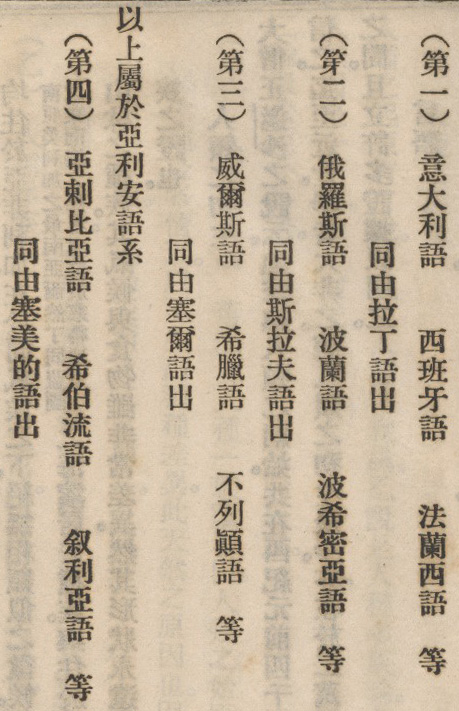
\includegraphics[height=8cm]{text14p32_2}
\end{tabular}

\begin{crossref}
For an example of a list-like structure without large spaces see \sect{section chinese tocs} (second example).
\end{crossref}


\subsubsection{Tables of Contents}
\label{section chinese tocs}

\mehrzeilen[5]

\begin{mainrule}
A table of contents is marked by §<toc>§ and §</toc>§. If the table of contents has a table-like structure or a list-like structure with large spaces, use §#§.
\end{mainrule}

\begin{clarification}
Type the §<toc>§ and §</toc>§ tags on separate lines. A table of contents may look like a table or like a list.
\end{clarification}

\vspace{3mm}
\begin{tabular}{@{}ll}
\parbox[b]{72mm}{
\htsc{Examples \\[2mm] \s{a table-like table of contents \\[2mm] a list-like table of contents \\ without large spaces}} \\[5mm]
\begin{typeChinese}
\f{<toc>} \\
\f{<h>}\z{第一章 天時}\f{</h>} \\
\z{日月} \f{\hash} \z{日月}\f{<}\z{蝕}\f{R>} \f{\hash} \z{地球} \f{\hash} \z{地球之圓體} \\
\z{地動說} \f{\hash} \z{遊星} \f{\hash} \z{七曜日} \f{\hash} \z{晝夜} \\
\z{時間} \f{\hash} \z{年月} \f{\hash} \z{歲首} \f{\hash} \f{<}\z{紀}\f{R>}\z{元} \\
\z{三時代} \f{\hash} \z{天氣豫報} \\
\f{<h>}\z{第二章 地理}\f{</h>} \\
\z{亞美利加} \f{\hash} \z{墺斯土剌利亞} \f{\hash} \z{蘇彛士河} \f{\hash} \z{山} \\
\z{堤埭} \f{\hash} \z{橋} \f{\hash} \z{周航地球} \f{\hash} \z{大洪水} \\
... \\
\f{</toc>} \\[28mm]
\end{typeChinese}
} & \qquad
\parbox[b]{5cm}{
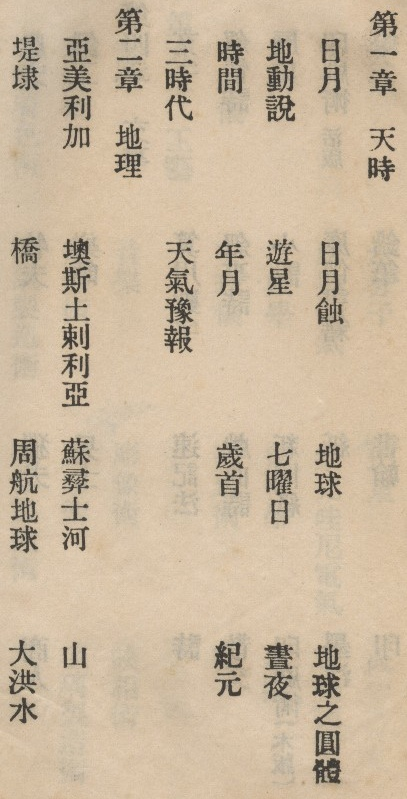
\includegraphics[height=8.5cm]{text14p5} \\[20mm] } \qquad
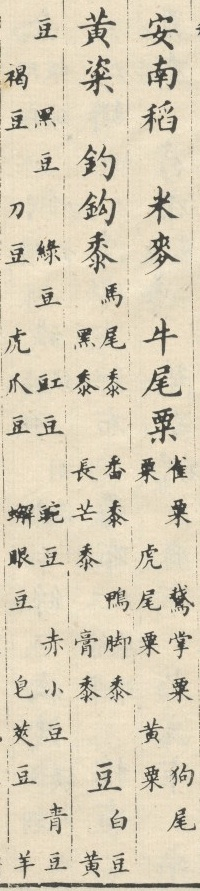
\includegraphics[height=11cm]{text17-1p7}
\end{tabular}

\vspace{-33mm}
\begin{typeChinese}
\f{<toc>} \\
... \\
\z{安南稻 米麥 牛尾粟}\f{<sm>}\z{雀粟 鵞掌粟 狗尾}\f{\bs\bs}\z{粟 虎尾粟 }\f{<}\z{黄}\f{V>}\z{粟}\f{</sm>} \\
\z{黄粢 釣鈎黍}\f{<sm>}\z{馬尾黍 番黍 鴨脚黍}\f{\bs\bs}\z{ 黑黍 長}\f{<}\z{芒}\f{R>}\z{黍 膏黍}\f{</sm>}\z{ 豆}\f{<sm>}\z{白豆}\f{\bs\bs}\z{ 黄} \\
\z{豆 黑豆 綠豆 豇豆 豌豆 赤小豆 青豆}\f{\bs\bs}\z{ 褐豆 刀豆 虎爪豆 蠏眼豆 皂}\f{<}\z{莢}\f{R>}\z{豆 羊} \\
... \f{</sm>} \\
\f{</toc>} \\
\end{typeChinese}


\tocspace
\subsection{Printed Images}


\subsubsection{Figures}
\label{section chinese figures}

\begin{mainrule}
Where a figure occurs in the text, type §<fig>§ on a separate line. If you can identify a caption of the figure, mark it by §<cap> </cap>§. Additional text that describes parts of the figure is marked by §<desc> </desc>§. Use a single §<var> </var>§ tag for variable names and numbers. Finally, type a closing §</fig>§ tag on a separate line.
%Figures are marked by §<fig>§ and §</fig>§ on separate lines. If you can identify a caption of the figure, mark it by §<cap> </cap>§. Additional text that describes parts of the figure is marked by §<desc> </desc>§. 
\end{mainrule}

\begin{clarification}
Type all §<cap>§, §<desc>§ and §<var>§ tags, in this order, on separate lines. A figure may have more than one description. If the same description is repeated in a figure, type it only once. Separate the variable names and numbers in the §<var> </var>§ by spaces. Type §<fig/>§ instead of §<fig>§ and §</fig>§ to mark simple figures without §<cap>§, §<desc>§ or §<var>§ tags.
%Type the caption on a separate line after §<fig>§. A figure may have more than one description. Type each description on a separate line after §<fig>§ and §<cap>§. If the same description is repeated in a figure, type it only once.
\end{clarification}

\begin{tabular}{@{}ll}
\parbox[b]{8.3cm}{
\htsc{Examples} \\
\begin{typeChinese}
\f{<fig>} \\
\f{<cap>}\z{第九鐵餅正看圖}\f{<sm>}\z{四分之一}\f{</sm>}\f{</cap>} \\
\f{<desc>}\z{秋}\f{</desc>} \\
\f{<desc>}\z{收}\f{</desc>} \\
\f{</fig>} \\
\f{<fig>} \\
\f{<cap>}\z{鐵餅剖看圖}\f{</cap>} \\
\f{<desc>}\z{秋}\f{</desc>} \\
\f{<desc>}\z{螺帽}\f{</desc>} \\
\f{<desc>}\z{收}\f{</desc>} \\
\f{<desc>}\z{螺鍵}\f{</desc>} \\
\f{</fig>} \\
\end{typeChinese}} &
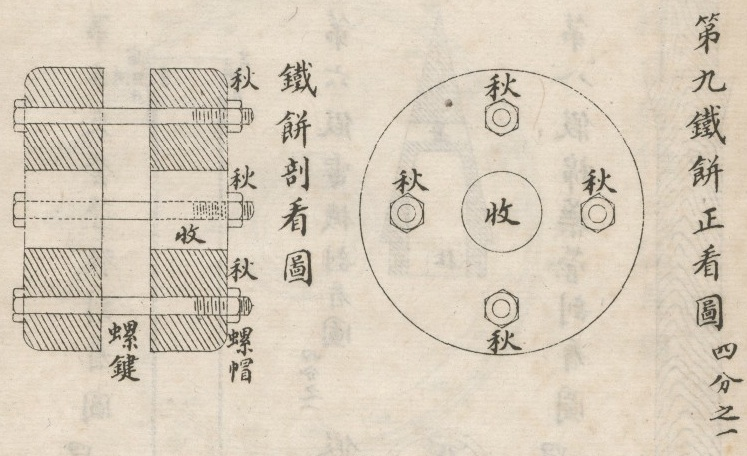
\includegraphics[width=8.1cm]{text18-1p24}
\end{tabular}

\vspace{5mm}
\begin{tabular}{@{}lll}
\parbox[b]{121mm}{
\begin{typeChinese}
\f{<fig>} \\
\f{<var>}\z{九} \z{甲} \z{六} \z{乙} \z{十二} \z{丙} \z{八} \z{丁}\f{</var>} \\
\f{</fig>} \\
\end{typeChinese}} & 
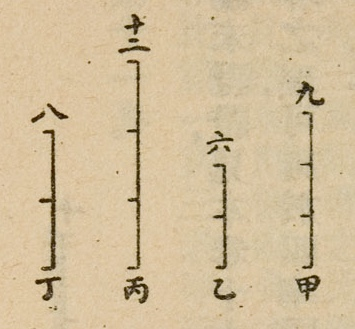
\includegraphics[height=4cm]{Euklid1996_p266}
\end{tabular}

\begin{tabular}{@{}lll}
\parbox[b]{126.5mm}{
\begin{typeChinese}
\\
\f{<pb a><rh>}\z{泰西事物}\f{<}\z{起}\f{V>}\z{原 }\f{<sm>}\z{第三章}\f{</sm></rh>} \\
... \\
\f{<fig>} \\
\f{<desc>}\z{第二大派}\f{</desc>} \\
\f{<desc>}\z{希伯流語}\f{</desc>} \\
\f{<desc>}\z{亞刺比亞語}\f{</desc>} \\ 
\\
\f{<pb b><rh>}\z{泰西事物起原 }\f{<sm>}\z{第三章}\f{</sm></rh>} \\
\f{<desc>}\z{非尼西亞語}\f{</desc>} \\
\f{</fig>} \\
... \\
\end{typeChinese}} & 
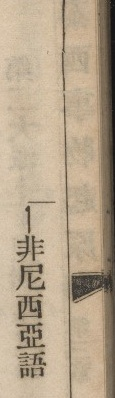
\includegraphics[height=5cm]{figure_14_33teil2} &
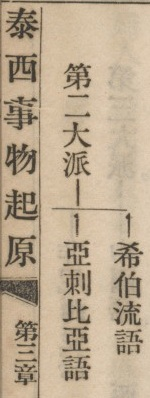
\includegraphics[height=5cm]{figure_14_33teil1}
\end{tabular}

\begin{tabular}{@{}lll}
\parbox[b]{8.3cm}{
\begin{typeChinese}
\f{<p>}\z{西洋大彈式十種 凡彈必合銃口徑以爲圓形故不預} \\
\z{定大小斤數}\f{</p>} \\
\f{<fig>} \\
\f{<desc>}\z{圓彈}\f{</desc>} \\
\f{</fig>} \\
\f{<fig>} \\
\f{<desc>}\z{中空}\f{<}\z{迎}\f{R>}\z{風} \\
\z{其聲如雷}\f{</desc>} \\
\f{<desc>}\z{響彈}\f{</desc>} \\
\f{</fig>} \\
\f{<fig>} \\
\f{<desc>}\z{中用百鍊鋼條兩頭銼} \\
\z{尖鑄時先定中}\f{<}\z{線}\f{R>}\z{毋使} \\
\z{稍偏長短致} \\
\z{有輕重低昂} \\
\z{不能直貫}\f{</desc>} \\
\f{<desc>}\z{遇賊攻} \\
\z{寨勢如} \\
\z{拉朽}\f{</desc>} \\
\f{</fig>} \\
\f{<fig>} \\
\f{<desc>}\z{彈形兩分中}\f{<}\z{綰}\f{R>}\z{百鍊} \\
\z{鋼條不拘長短點放} \\
\f{<}\z{迸}\f{R>}\z{發橫拉如火龍}\f{</desc>} \\
\f{<desc>}\z{鍊彈}\f{</desc>} \\
\f{</fig>} \\
\f{<fig>} \\
\f{<desc>}\z{最厚之城用十}\f{<}\z{餘}\f{R>}\z{彈先} \\
\z{鑿破磚石}\f{<}\z{繼}\f{R>}\z{以員彈推} \\
\z{倒}\f{</desc>} \\
\f{<desc>}\z{攻城}\f{</desc>} \\
\f{</fig>} \\
\f{<fig>} \\
\f{<desc>}\z{攻城攻墻一也特中用} \\
\z{鋼鑿大小厚薄不同耳} \\
\z{鑄法如前說}\f{</desc>} \\
\f{<desc>}\z{攻墻}\f{</desc>} \\
\f{</fig>} \\
\end{typeChinese}
} & 
\parbox[b]{8cm}{
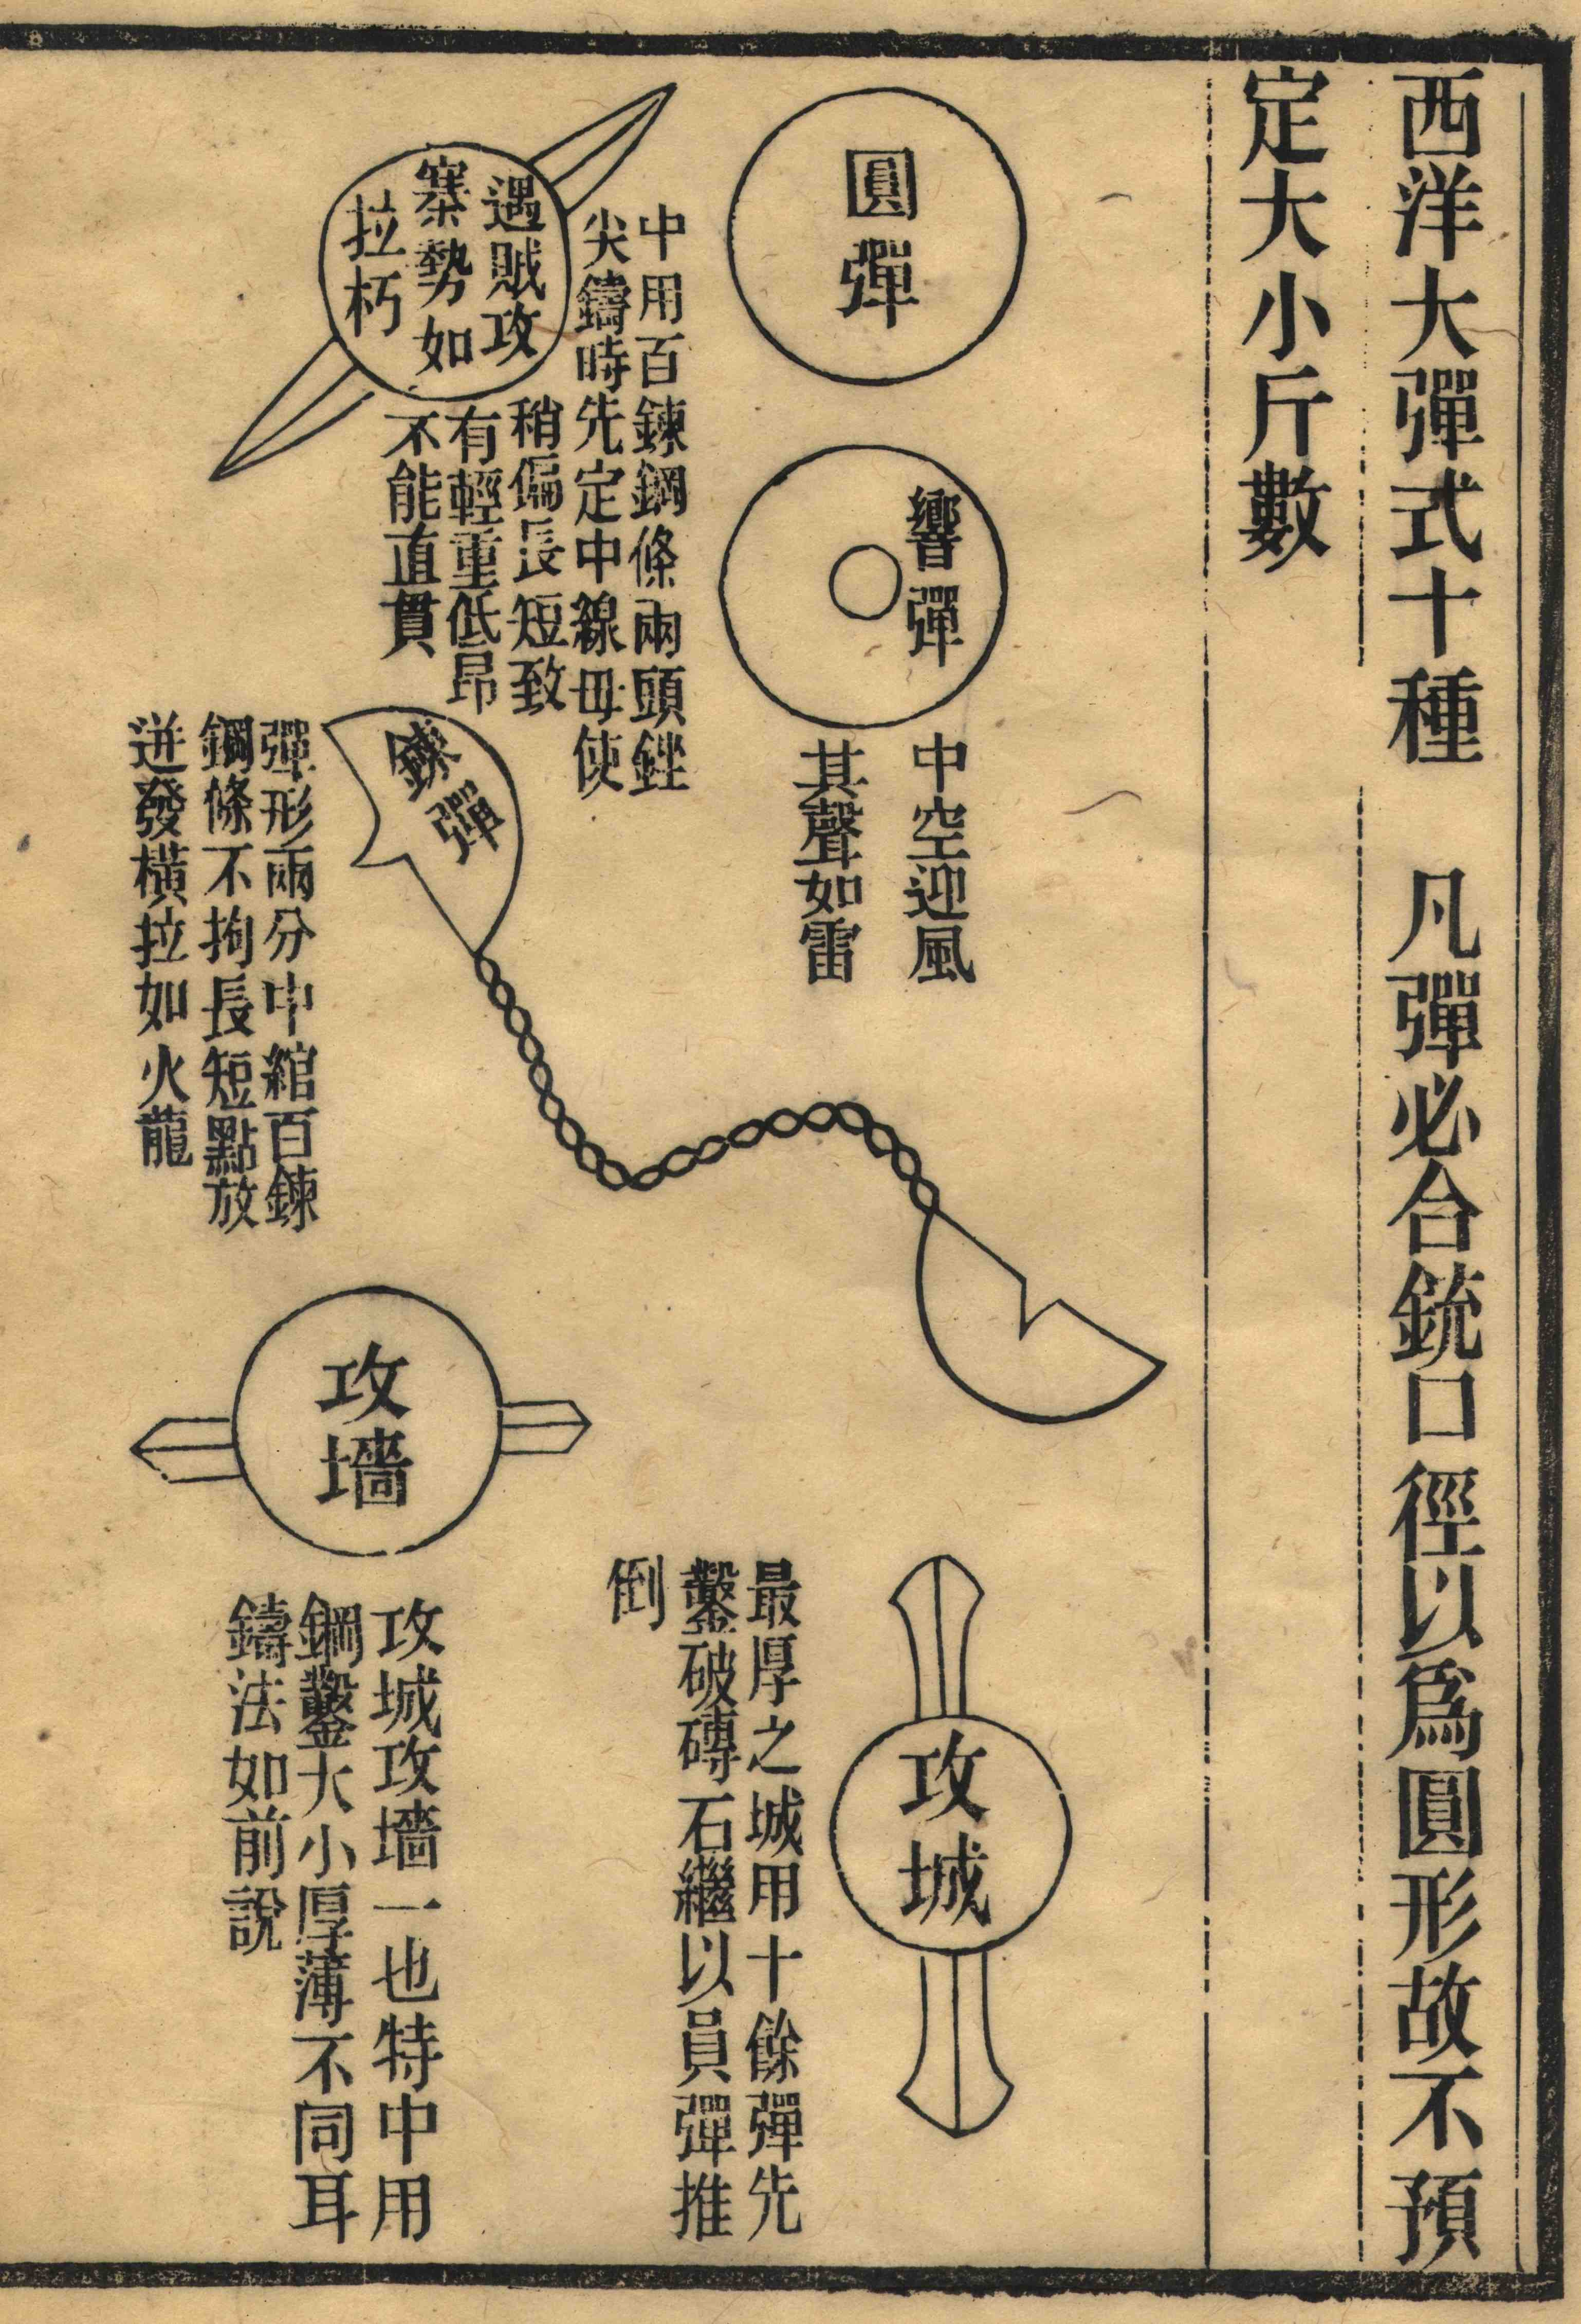
\includegraphics[height=12cm]{text16p69} 
\vspace{14mm}
\\
}
\end{tabular}


\subsubsection{Stamps}
\label{section chinese stamps}

\begin{mainrule}
Stamps are marked by §<stamp>§. Type the §<stamp>§ tag on a separate line. Do not type the text in the stamp.
\end{mainrule}

\begin{crossref}
For an example see \sect{section chinese headings}.
\end{crossref}


\tocspace
\subsection{Unreadable Text}
\label{section unreadable text}


\subsubsection{Characters You are Unsure About}
\label{section characters you are unsure about}

\begin{mainrule}
If you are not sure about a character, type §<?>§ after it. If you are unsure about a whole paragraph, type §<?>§ directly after the §<p>§ tag, i.e. §<p><?>§. A completely unreadable character is typed as §@§. If many characters are unreadable, use §<gap>§ instead of §@§.
\end{mainrule}

\begin{clarification}
Use one §@§ for each unreadable character, e.g. §unr@@dable§. If in doubt, use §<gap>§, e.g. §unr<gap>dable§. If you are unsure about a group of characters, for example a whole word, do not type §<?>§ repeatedly for every character, e.g. type §word<?>§ rather than §w<?>o<?>r<?>d<?>§.
\end{clarification}

\begin{tabular}{@{}ll}
\parbox[b]{129.5mm}{
\htsc{Examples} \\[8mm]
\begin{typeChinese}
\z{上戊其日祀事禮成}\f{<?>@} \\
\z{陳尚明率元儒姬紹周}\f{<?>} \\[5mm]
\f{<dl>}\z{古禮}\f{</dl><?>}\z{德}\f{<}\z{運}\f{R>}\z{河之間。} \\[7mm]
\end{typeChinese}
} &
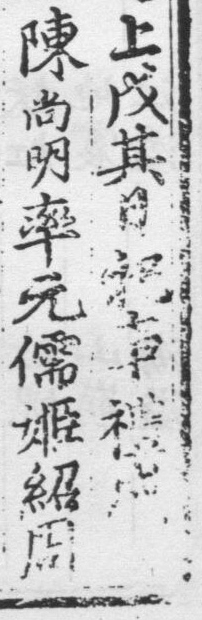
\includegraphics[height=5cm]{unreadable} \quad
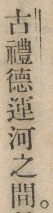
\includegraphics[height=5cm]{text14p74_unclear} 
\end{tabular}

\begin{note}
In the second example, the characters are readable but the double line (see \sect{section chinese underlinings}) is badly printed.
\end{note}

\begin{crossref}
For unknown rather than unreadable characters please refer to \sect{section unknown characters}. 
\end{crossref}


\subsubsection{Unknown Characters}
\label{section unknown characters}

\begin{mainrule}
If there is an unknown character in the text, i.e. a character variant which is readable but where you cannot identify the standard character, add it to the numbered list of unknown characters. From then on, type its number whenever it occurs in the text, e.g. §<001>§.
\end{mainrule}
 
\begin{clarification}
Before you create a number for an unknown character, first check whether it is already on the list of unknown characters. Assign the number §<001>§ to the first unknown character, §<002>§ to the second unknown character, and so on. Do not assign the same number twice. Use this number to type the unknown character. Always use the same number if the same unknown character occurs again. 
\end{clarification}

\begin{note}
Make sure that for a given text there is a single list containing all unknown characters, and that everyone uses this list. When the text is sent back to us, we will need a copy of this list. (See also \sect{section file conventions}.)
\end{note}

\begin{tabular}{@{}ll}
\parbox[b]{145.5mm}{
\htsc{Example \\[2mm] \s{an unknown character}} \\[15mm]
\begin{typeChinese}
\f{<}\z{得}\f{V>}\z{梁}\f{<001>}\z{玉}\f{<}\z{虎}\f{V><}\z{枕}\f{V>} \\[7mm]
\end{typeChinese}
} & \qquad
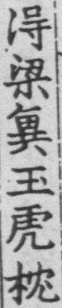
\includegraphics[height=5cm]{unknown_chinese_character2}
\end{tabular}

\vspace{3mm}
\begin{crossref}
For unreadable rather than unknown characters please refer to \sect{section characters you are unsure about}. For §< V>§, i.e. if a character variant is not included in Unicode but you can identify the standard character, see \sect{section character variants}.
\end{crossref}

\vspace{3mm}
\begin{note}
%§<001>§ is actually an unusual version of the variant \z{兾} of the character \z{冀}. If you can identify it as a version of the character variant, mark it as §<§\z{兾}§V>§ instead of §<001>§. If you cannot identify the variant but you can identify the standard character, mark it as §<§\z{冀}§V>§.
§<001>§ is actually an unusual version of the variant \z{兾} of the character \z{冀}. If you can identify the standard character \z{冀}, mark it as §<§\z{冀}§V>§ instead of §<001>§. 

If in addition you can identify it as a version of the character variant \z{兾} (i.e. as a version of a character variant with a separate Unicode codepoint), mark it as §<§\z{兾}§V>§. (This special case is not mentioned in \sect{section character variants}.)
\end{note}


\tocspace
\section{Chinese Characters}

\tocspace
\subsection{General}

\subsubsection{Punctuation}
\label{section chinese punctuation}

\begin{mainrule}
Type the punctuation to the right of characters.
\end{mainrule}

\begin{crossref}
For an example see \sect{section chinese paragraphs}.
\end{crossref}


\subsubsection{Spaces}

\begin{mainrule}
Type spaces in Chinese text as the IDEOGRAPHIC SPACE character U+3000.
\end{mainrule}

\begin{clarification}
In running heads (§<rh>§, see \sect{section page breaks}) and headings (§<h>§ and §<ti>§, see \sect{section chinese headings}), type large spaces as a single ideographic space character.
In tables and lists (§<tb>§, §<list>§ and §<toc>§, see \sect{section structured text}), use §#§ for large spaces.
\end{clarification}

\begin{clarification}
If you encounter a large space in a normal paragraph (§<p>§, see the example in \sect{section chinese paragraphs}, third line from the bottom), make sure that none of the cases above apply. If it is indeed a normal paragraph, type the large space as more than one ideographic space, according to its length. 
\end{clarification}

\begin{crossref}
For an example of large spaces that are typed as a single ideographic space character, see \sect{section page breaks}. For an example of large spaces that are typed as §#§, see \sect{section tables}.
\end{crossref}


\tocspace
\subsection{Character Variants}
\label{section character variants}


\subsubsection{Character Variants and Unicode}
\label{section character variants and unicode}

\begin{mainrule}
If a character variant is included in Unicode 5.1, type it. Do not normalize the variant.
%The rest of this section applies only to characters which are not included in Unicode.
\end{mainrule}

\begin{clarification}
For example, if the character variant \z{歴} of the character \z{歷} occurs in the text, type \z{歴} (U+6B74).
%\end{clarification}
%
%\begin{clarification}
Rather than working with the reference glyphs of the Unicode codepoints, you may use the fonts Sun-ExtA and Sun-ExtB normatively.
\end{clarification}

\vspace{5mm}
\begin{mainrule}
If a character variant is not included in Unicode 5.1, type the standard character instead. In addition, mark it by §< R>§ or §< V>§ if the rules in \sect{section rules for marking character variants} apply.
\end{mainrule}

\begin{crossref}
If you cannot identify the standard character, treat it as unknown character (see \sect{section unknown characters}).
\end{crossref}

\begin{clarification}
If a character variant should be marked, add it to the Character Variants List, i.e. add the image and how you have marked it. In addition, mark the first occurrence of the character variant in the text. After its first occurrence, silently normalize it. Begin a new Character Variants List for each text. 
\end{clarification}

\begin{note}
In rare cases, the same text may contain the standard character and one or more different variants of this character. Please make a note in the Character Variants List, e.g. “S + V” or “V1 + V2” or “S + V1 + V2”. Include an image of each variant. In the text, mark the first occurrence of each variant using §< V1>§, §< V2>§, etc. Do not mark the standard character.
\end{note}

%\vspace{5mm}
\subsubsection{Rules for Marking Character Variants}
\label{section rules for marking character variants}

This sections contains \textsf{\textbf{Rule S}} for simple differences that need not be marked, \textsf{\textbf{Rule R}} for marking old radicals, and \textsf{\textbf{Rule V}} for other variations. 

\begin{mainrule}
\paragraph{Rule S (silently normalizing simple differences):} If a character variant differs from the standard character only in the following points, type it as the standard character and do not mark the difference. 
\end{mainrule}

\begin{clarification}
In paragraphs with individualized character style (see \sect{section individualized character style}) and in handwritten text (see \sect{section handwritten text}), silently normalize character variants if they are not in Unicode.
\end{clarification}

%\vspace{2mm}
%\begin{liste}[ 1: \, normalizations (from ISO 10646, slightly modified)]
%\begin{longtable}{@{}l@{ }ll} \\
%& Description & Examples \\[2mm]
%a) & Differences in rotated strokes/dots & 
\includegraphics{iso-a} \\
%b) & \parbox[t]{8cm}{Differences in overshoot at the stroke initiation and/or termination} & \includegraphics{iso-b} \\
%c) & \parbox[t]{8cm}{Differences in contact of strokes} & 
\includegraphics{iso-c} \\
%d) & \parbox[t]{8cm}{Differences in protrusion at the folded corner of strokes} & 
\includegraphics{iso-d} \\
%e) & \parbox[t]{8cm}{Differences in bent strokes} & 
\includegraphics{iso-e} \\
%f) & \parbox[t]{8cm}{Differences in folding back at the stroke termination} & 
\includegraphics{iso-f} \\
%g) & \parbox[t]{8cm}{Differences in accent at the stroke initiation} & 
\includegraphics{iso-g} \\
%h) & \parbox[t]{8cm}{Differences in “rooftop” modification} & 
\includegraphics{iso-h} \\
%i) & \parbox[t]{8cm}{Straightforward combinations of the above differences} & 
\includegraphics{iso-j} \\
%\end{longtable}
%\end{liste}

% Version aus 2.0.1:
%\vspace{3mm}
%\begin{liste}[: \, simple differences the need NOT be marked \, (from ISO 10646, slightly modified)]
%\begin{longtable}{@{}l@{ }ll} 
%& Description & Examples \\[5mm]
%a) & Differences in rotated strokes/dots & \parbox[m]{8cm}{ 
\includegraphics{iso-a} } \\[5mm]
%b) & \parbox[m]{8cm}{Differences in overshoot at the stroke initiation and/or termination} & \parbox[m]{8cm}{ 
\includegraphics{iso-b2}  } \\[5mm]
%c) & \parbox[t]{8cm}{Differences in contact of strokes} & \parbox[m]{8cm}{ 
\includegraphics{iso-c}  } \\[5mm]
%d) & \parbox[m]{8cm}{Differences in protrusion at the folded corner of strokes} & \parbox[m]{8cm}{ 
\includegraphics{iso-d}  } \\[5mm]
%e) & \parbox[t]{8cm}{Differences in bent strokes} & \parbox[m]{8cm}{ 
\includegraphics{iso-e}  } \\[5mm]
%f) & \parbox[m]{8cm}{Differences in folding back at the stroke termination} & \parbox[m]{8cm}{ 
\includegraphics{iso-f}  } \\[5mm]
%g) & \parbox[m]{8cm}{Differences in accent at the stroke initiation} & \parbox[m]{8cm}{ 
\includegraphics{iso-g}  } \\[5mm]
%h) & \parbox[t]{8cm}{Differences in “rooftop” modification} & \parbox[m]{8cm}{ 
\includegraphics{iso-h}  } \\[5mm]
%i) & \parbox[m]{8cm}{Straightforward combinations of the above differences} & \parbox[m]{8cm}{ 
\includegraphics{iso-j}  } \\[5mm]
%\end{longtable}
%\end{liste}


%& \multicolumn{2}{@{}l}{\parbox[m]{16cm}{Do not mark \includegraphics{chin21zhi} (\z{之}) where the dot at the top touches or even overshoots the horizontal stroke. }} \\[5mm]
%& \multicolumn{2}{@{}l}{\parbox[m]{16cm}{Similarly, do not mark the difference between \includegraphics{chin21zhi} CHI and \z{斥} .}} \\[10mm]
%& \multicolumn{2}{@{}l}{\parbox[m]{16cm}{However, DO mark the difference between \z{亠} and \z{十} and between \z{卜} and \z{十}. Examples:  \includegraphics{chin21zhi} HUAI  <\z{櫰}V>,  \includegraphics{chin21zhi} FEI  <\z{肺}V>.}} \\[10mm]

\vspace{3mm}
\begin{liste}[: \, simple differences \, (with excerpts from ISO 10646)]

a) Differences in rotated strokes/dots

\begin{itemize}
\item[‒] Do NOT mark \,\parbox{8cm}{ 
\includegraphics{iso-a} }

\item[‒] Do NOT mark 
\parbox{9mm}{ 
\includegraphics{chin21a1} } (\z{之}) 
where the dot at the top touches or even overshoots the horizontal stroke. 
Similarly, do not mark the difference between 
\parbox{8mm}{ 
\includegraphics{chin21a2} } and \z{斥}.

\vspace{2mm}
\item[+] DO mark the difference between \z{亠} and \z{十} and between \z{卜} and \z{十}. \\ Examples: \,
\parbox{8mm}{ 
\includegraphics{chin21a3} } <\z{櫰}V>, 
\parbox{10mm}{ 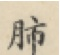
\includegraphics{chin21a4} } <\z{肺}V>.
\end{itemize}

\vspace{5mm}
b) Differences in overshoot at the stroke initiation and/or termination

\begin{itemize}
\item[‒] Do NOT mark \,\parbox{8cm}{ 
\includegraphics{iso-b2} }

\item[‒] Do NOT mark 
\parbox{9mm}{ 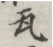
\includegraphics{chin21b1} } (\z{瓦}), 
\parbox{8mm}{ 
\includegraphics{chin21b2} } (\z{耶}), or 
\parbox{9mm}{ 
\includegraphics{chin21b4} } (\z{承}). 
Also do not mark 
\parbox{9mm}{ \includegraphics{chin21b5} } (\z{皴}), 
i.e. the differences in the overshot/non-overshot of the character part \z{夕}.

\vspace{2mm}
\item[+] DO mark vertical (\z{竪}) and left-slanted (\z{撇}) overshoots. \\
Examples: \,
\parbox{9mm}{ \includegraphics{chin21b6} } <\z{割}V>, 
\parbox{7mm}{ \includegraphics{chin21b7} } <\z{除}V>, 
\parbox{10mm}{ \includegraphics{chin21b8} } <\z{楔}V>, 
\parbox{10mm}{ \includegraphics{chin21b9} } <\z{鄂}V>, 
\parbox{9mm}{ \includegraphics{chin21b10} } <\z{蛇}V>.
\end{itemize}

\vspace{5mm}
c) Differences in contact of strokes

\begin{itemize}
\item[‒] Do NOT mark \,\parbox{8cm}{ \includegraphics{iso-c} }

\item[+] DO mark connections of the vertical strokes of the component \z{日} with a horizontal stroke \z{一} below that look like a change from \z{旦} to \z{且}. \\
Example: The component \z{昜} in 
\parbox{9mm}{ \includegraphics{chin21c1} } <\z{盪}V>.
%\includegraphics{chin21c1test.pdf} <\z{盪}V>.
\end{itemize}

\vspace{5mm}
d) Differences in protrusion at the folded corner of strokes

\begin{itemize}
\item[‒] Do NOT mark \,\parbox{8cm}{ \includegraphics{iso-d} }

\item[‒] Do NOT mark 
\parbox{7mm}{ \includegraphics{chin21d1.pdf} } (\z{繩}) or
\parbox{7mm}{ \includegraphics{chin21d2.pdf} } (\z{斲}).

\item[‒] Do NOT mark the difference between the character components \z{已} (\textit{ji} “self”) and \z{己} (\textit{yi} “already”) unless you are completely sure.

\item[+] DO mark the difference between \z{巳} 
%(\textit{si}, Earthly Branch “snake”) 
and \z{已} / \z{己}. \\
Examples: \,
\parbox{7.5mm}{ \includegraphics{chin21d3.pdf} } <\z{忌}V>,
\parbox{9mm}{ \includegraphics{chin21d4.pdf} } <\z{包}V>.

\item[+] DO mark the difference between \z{㔾} and \z{巳} and the difference between \z{皿} and \z{罒}. \\
Examples: \,
\parbox{8mm}{ \includegraphics{chin21d5.pdf} } <\z{卷}V>, 
\parbox{7mm}{ \includegraphics{chin21d6.pdf} } <\z{服}V>, 
\parbox{7mm}{ \includegraphics{chin21d7.pdf} } <\z{衆}V>.
\end{itemize}

\vspace{5mm}
e) Differences in bent strokes

\begin{itemize}
\item[‒] Do NOT mark \,\parbox{8cm}{ \includegraphics{iso-e} }

\item[+] DO mark the difference between \z{巜} and \z{刂} and the difference between \z{术} and \z{朮}. In general, mark differences in the shape of a stroke if they lead to a different character component. \\
Examples: \,
\parbox{7mm}{ \includegraphics{chin21e1.pdf} } <\z{俞}V>, 
\parbox{8mm}{ \includegraphics{chin21e2.pdf} } <\z{述}V>.
\end{itemize}

\vspace{5mm}
f) Differences in folding back at the stroke termination

\begin{itemize}
\item[‒] Do NOT mark \,\parbox{8cm}{ \includegraphics{iso-f} }
\end{itemize}

\vspace{5mm}
g) Differences in accent at the stroke initiation

\begin{itemize}
\item[‒] Do NOT mark \,\parbox{8cm}{ \includegraphics{iso-g} }
\end{itemize}

\vspace{5mm}
h) Differences in “rooftop” modification

\begin{itemize}
\item[‒] Do NOT mark \,\parbox{8cm}{ \includegraphics{iso-h} }

\item[‒] Do NOT mark for example 
\parbox{7mm}{ \includegraphics{chin21h1.pdf} } (\z{肉}).

\item[+] DO mark the difference between \z{几} and \z{儿}. \\
Examples: \,
\parbox{8mm}{ \includegraphics{chin21h2.pdf} } <\z{兜}V>, 
\parbox{7mm}{ \includegraphics{chin21h3.pdf} } <\z{虎}V>.
\end{itemize}

\vspace{5mm}
i) Straightforward combinations of the above differences

\begin{itemize}
\item[‒] Do NOT mark \,\parbox{8cm}{ \includegraphics{iso-j} }
\end{itemize}

\end{liste}

\vspace{3mm}
\begin{note}
The rules a) to i) leave the number of strokes unchanged. Consequently, changes in the number of strokes cannot be silently normalized and must be marked.

\vspace{2mm}
Note, however, that in some printing styles the strokes \extB{𠄌} (\textit{shuti} \z{竪提}) and \extB{𠃊} (\textit{shuzhe} \z{竪折}) appear to be a combination of two strokes, i.e. “vertical” (\z{丨}) plus “upward-slanted” (\z{㇀}). Do not mark these printing styles. \\
Examples: \,
\parbox{7mm}{ \includegraphics{chin21n1.pdf} } (\z{裏}),
\parbox{9mm}{ \includegraphics{chin21n2.pdf} } (\z{震}),
\parbox{6.5mm}{ \includegraphics{chin21n3.pdf} } (\z{改}),
\parbox{7mm}{ \includegraphics{chin21n4.pdf} } (\z{粵}),
\parbox{10mm}{ \includegraphics{chin21n5.pdf} } (\z{仰}).
\end{note}

\begin{mainrule}
\paragraph{Rule R (marking old radicals):} If a character such as \z{絨} (U+7D68) exists in Unicode 5.1 only with the new shape \z{糹} (U+7CF9) of the radical (\emph{bushou} \z{部首}) and not with the old shape \z{糸} (U+7CF8), mark the character variant with the old radical by §< R>§, for example §<§\z{絨}§R>§. Apply this rule only if the difference between the old and the new radical is not covered by rule S.
\end{mainrule}

\begin{crossref}
Appendix \ref{appendix radicals} contains a list of radicals that need to be marked.
\end{crossref}

\begin{note}
%The most significant examples of this rule are those where a graphem originally belonging to the sound-part of a character took over a graphical position that normally belongs to a radical while the actual radical of the character is "swallowed" by the sound-part. \\
%Rule R also applies when a character component has moved from the sound-part of the character to the radical part. \\
Rule R also applies when a character component from the sound-part of the character has swapped places with the actual radical. \\
Examples: \,
\parbox{10mm}{ \includegraphics{chin21r1.pdf} } <\z{穫}R>,
\parbox{5mm}{ \includegraphics{chin21r2.pdf} } <\z{墜}R>.
\end{note}

%\vspace{5mm}
\begin{mainrule}
\paragraph{Rule V (marking other variations):} If the non-radical part of the character variant differs from that of the standard character, mark the character variant with §< V>§. Apply this rule only if the difference is not covered by rule S.
\end{mainrule}

%\vspace{5mm}
%\begin{tabular}{@{}ll}
%\parbox[b]{134mm}{
%\htsc{Example \\[2mm] \s{a character variant with an additional stroke}}  \\[-2mm]
%\begin{typeChinese}
%\f{<}\z{彈}\f{V>} \\
%\end{typeChinese}
%} & \qquad
% \includegraphics[height=2cm]{variante} 
%\end{tabular}

%\begin{tabular}{@{}ll}
%\parbox[b]{139.5mm}{
%\htsc{Example \\[2mm] \s{a character variant not included in Unicode 5.1.0}} \\[15mm]
%\begin{typeChinese}
%\z{郡兩}\f{<}\z{穫}\f{V>}\z{者} \\[7mm]
%\end{typeChinese}
%} & \qquad
%\includegraphics[height=5cm]{text17-1p15_klein}
%\end{tabular}

\vspace{3mm}
\begin{tabular}{@{}ll}
\parbox[b]{122.5mm}{
\htsc{Examples} \\[15mm]
\begin{typeChinese}
\f{<}\z{彈}\f{V>} \\[5mm]
\z{郡兩}\f{<}\z{穫}\f{R>}\z{者} \\[5mm]
\end{typeChinese}
} &
\includegraphics[height=1.5cm]{variante}  \qquad
\includegraphics[height=5cm]{text17-1p15_klein}
\end{tabular}

\vspace{2mm}
\begin{clarification}
If both rule R and rule V apply, mark the character variant by §< RV>§; see the example §<§\z{過}§RV>§ in \sect{section chinese paragraphs}.
\end{clarification}


\tocspace
\subsection{Type Styles}

\subsubsection{Small Characters}
\label{section chinese small characters}

\begin{mainrule}
Strings of small characters are marked by §<sm> </sm>§. Indicate half-column breaks by §\\§. 
\end{mainrule}

\begin{crossref}
For an example see \sect{section chinese tocs} (second example). This examples includes strings of small characters over more than one line of text.
\end{crossref}


%\mehrzeilen[3]

\subsubsection{Underlinings}
\label{section chinese underlinings}
  
\begin{mainrule}
A single line next to characters is marked by §<sl> </sl>§. 
A double line next to characters is marked by §<dl> </dl>§. 
A circled line next to characters is marked by §<cl> </cl>§.
A wavy line next to characters is marked by §<wl> </wl>§.
\end{mainrule}

\begin{note}
In old texts, the lines are to the right of characters. In modern texts, the lines may also be to the left of characters. The position to the left or right is not encoded.
\end{note}

\begin{tabular}{@{}ll}
\parbox[b]{139mm}{
\htsc{Example \\[2mm] \s{underlinings to the left and right}} \\[15mm]
\begin{typeChinese}
\f{<sl>}\z{康熙}\f{</sl><wl>}\z{寶應縣志}\f{</wl>}\z{人物志: 柏叢桂} \\
\z{有司寢不行。}\f{<cl><sl>}\z{叢桂}\f{</sl>}\z{更相度地形畫圖}\f{</cl>}\z{。} \\[12mm]
\end{typeChinese}
} & \qquad
\includegraphics[height=6cm]{Specs-Bild1_2}
\end{tabular}

\begin{crossref}
For an example with underlinings to the right of characters see \sect{section chinese paragraphs}. This example includes §<dl>§ for double lines.
\end{crossref}

\newpage
\subsubsection{Individualized Character Style}
\label{section individualized character style}

\begin{mainrule}
A paragraph in an individualized character style is marked by §ics§ in the §<p>§ tag, i.e. §<p ics>§. 
\end{mainrule}

\begin{clarification}
If a character variant in a §<p ics>§ paragraph is not in Unicode, resolve it silently, i.e. do not use §< V>§ or §< R>§. However, use §<001>§ if a character is unknown.
\end{clarification}

\begin{tabular}{@{}ll}
\parbox[b]{138.5mm}{
\htsc{Example} \\[5mm]
\begin{typeChinese}
\f{<p ics>}\z{光緒十六年} \\
\z{冬印扵天津} \\
\z{李鴻章署检}\f{</p>} \\[5mm]
\end{typeChinese}
} &
\includegraphics[height=4cm]{text18-1p2}
\end{tabular}


\subsubsection{Handwritten Text}
\label{section handwritten text}

\begin{mainrule}
%%If a character has been crossed out, mark it by §{ }§. 
%%If there is a corrected character next to the crossed-out character, mark this by §{ / }§. 
%%If there is a line between two consecutive characters indicating that the order should be reversed, mark this by §{ ~ }§, but type the characters in the order as they appear in the text.
%If a character has been crossed out, mark it by §{ -}§. e.g.  §{§\z{四}§-}§.
%If there is a corrected character next to the crossed-out character, mark this by §{ - }§, e.g. §{§\z{四}§-§\z{五}§}§. If one character has been written on top of another character and the original character is no longer readable, mark it by §{- }§, e.g. §{@-§\z{五}§}§.
%If there is a line between two consecutive characters indicating that the order should be reversed, mark this by §{ ~ }§, but type the characters in the order as they appear in the text.
If a character has been crossed out, mark it by §{ /}§, e.g.  §{§\z{四}§/}§. If a character has been inserted, mark it by §{ }§, e.g. §{§\z{五}§}§. If the inserted character replaces a crossed-out character, mark this by §{§\z{四}§/§\z{五}§}§, or  §{@/§\z{五}§}§ if the crossed-out character is no longer readable.
\end{mainrule}

\begin{mainrule}
If there is a line between two consecutive characters indicating that the order should be reversed, mark this by §{ ~ }§, but type the characters in the order as they appear in the text.
\end{mainrule}

\begin{clarification}
If a character variant in handwritten text is not in Unicode, resolve it silently, i.e. do not use §< V>§ or §< R>§. However, use §<001>§ if a character is unknown.
\end{clarification}

\vspace{3mm}
\begin{tabular}{@{}ll}
\parbox[b]{56mm}{
\htsc{Examples} \\[6mm]
\begin{typeChinese}
\z{均}\f{\{}\z{的加减号於次均}\f{\}}\z{旁又随錄} \\[5mm]
\z{行內}\f{\{}\z{倒}\f{/}\z{减}\f{\}}\z{去} \\[2mm]
\z{維}\f{\{@/}\z{揚}\f{\}}\z{人家} \\[5mm]
\f{\{}\z{左}\f{\tld}\z{其}\f{\}} \\
\end{typeChinese}
} &
\includegraphics[height=5cm]{tian_p18} \qquad
\includegraphics[height=5cm]{hd_tian_p23} \,\,
\includegraphics[height=5cm]{yin1_p27} \qquad
\includegraphics[height=5cm]{xing_jing_p39}
\end{tabular}

%\begin{tabular}{@{}ll}
%\parbox[b]{8cm}{
%\htsc{Examples} \\[25mm]
%\begin{typeChinese}
%xx\bold{\{}x\bold{\}}xx \\ \\
%xxxx\{x/x\}\{x/x\}xx \\ \\
%xx\bold{\tld}xxx \\ 
%\end{typeChinese}
%} & \qquad
%\includegraphics[height=6cm]{Specs-Bild2-kt}
%\end{tabular}

%%Or something like §<del>x</del>§, §<repl>xx</repl>§ and §<rev>xx</re>§?

\appendix

\newpage
\section{Old Radicals That Need to be Marked}
\label{appendix radicals}

\begin{note} 
This list is only a guideline and may not be complete.
\end{note}

An entry such as \hira{⺿} \z{⻀} §(§\z{⺾}§)§ means that if a character has \hira{⺿} or \z{⻀} as the shape of its radical, and the character with this variant radical is not included in Unicode 5.1, type the standard character and add §< R>§. 
Example: §<§\z{蒼}§R>§.

Example of a radical that does not have to be marked: Do not mark the old shape \mincho{爫} of the radical \z{爫} because of point a) in the list in \sect{section rules for marking character variants}.

\vspace{3mm}
\begin{liste}[: \, old radicals that need to be marked]
\begin{tabular}{@{}l@{ }lll@{ }lll@{ }lll@{ }l} \\
\z{彑} & §(§\z{彐}§)§ &&
\z{糸} & §(§\z{糹}§)§ &&
\z{⻞} & §(§\z{⻟}§)§ &&
\sunExtB{𦈢} & §(§\z{缶}§)§ \\[2mm]
\sunExtB{𦣞} & §(§\z{臣}§)§ &&
\z{襾} & §(§\z{西}§)§ &&
\sunExtB{𧢲} & §(§\z{角}§)§ &&
\sunExtB{𧰧} & §(§\z{豕}§)§ \\[2mm]
\z{赱} & §(§\z{走}§)§ &&
\sunExtB{𨑄𨑃} & §(§\z{辰}§)§ &&
\mincho{辶} & §(§\z{辶}§)§ &&
\z{采} & §(§\z{釆}§)§ \\[2mm]
\z{镸} & §(§\z{長}§)§ &&
\sunExtA{门}\sunExtB{𨳇} & §(§\z{門}§)§ &&
\sunExtB{𨸏} & §(§\z{阝}§)§ &&
\z{靑} & §(§\z{青}§)§ \\[2mm]
\sunExtA{靣}\sunExtB{𠚑} & §(§\z{面}§)§ &&
\z{凬} & §(§\z{風}§)§ &&
\sunExtB{𩙱} & §(§\z{飛}§)§ &&
\sunExtB{𩙿𩚁} & §(§\z{飠}§)§ \\[2mm]
\sunExtB{𩠐} & §(§\z{首}§)§ &&
\sunExtB{𩡧} & §(§\z{馬}§)§ &&
\z{髙} & §(§\z{高}§)§ &&
\sunExtB{𩵋} & §(§\z{魚}§)§ \\[2mm]
\sunExtB{𠧸} & §(§\z{鹵}§)§ &&
\sunExtB{𢉖} & §(§\z{鹿}§)§ &&
\z{黃} & §(§\z{黄}§)§ &&
\z{黒} & §(§\z{黑}§)§ \\[2mm]
\sunExtB{𪗄} & §(§\z{⿑}§)§ &&
\z{歯} & §(§\z{齒}§)§ &&
\sunExtB{𪛉𪚦} & §(§\z{⿔}§)§ &&
\hira{⺿} \z{⻀} & §(§\z{⺾}§)§ \\
\end{tabular}
\end{liste}

\newpage
\section{List of All Tags}
\label{appendix list of all tags}

\begin{longtable}[l]{@{}llll@{}l@{}}
section & tag & name & tag may contain \\[1mm]
\hline \\
\ref{section page breaks} & §<pb>§ & page break & page number, a/b \\
\ref{section page breaks} & §<rh> </rh>§ & running head &\\
\\
\ref{section chinese headings} & §<h> </h>§ & heading & level number \\
\ref{section chinese headings} & §<ti> </ti>§ & \emph{ti} \z{題} &\\
\ref{section chinese paragraphs} & §<p> </p>§ & paragraph & §i§, §x§, §ics§ \\
\\
\ref{section tables} & §<tb> </tb>§ & table &\\
\ref{section tables} & §#§ & field separator \\
\ref{section chinese lists} & §<list> </list>§ & list &\\
\ref{section chinese tocs} & §<toc> </toc>§ & table of contents &\\
\\
\ref{section chinese figures} & §<fig> </fig>§ & figure & \\
\ref{section chinese figures} & §<cap> </cap>§ & figure caption &\\ 
\ref{section chinese figures} & §<desc> </desc>§ & figure description &\\ 
\ref{section chinese figures} & §<var> </var>§ & figure variables &\\ 
\ref{section chinese stamps} & §<stamp> </stamp>§ & stamp & \\
\\
\ref{section characters you are unsure about} & §<?>§ & uncertain text & \\
\ref{section characters you are unsure about} & §@§, §<gap>§ & unreadable text & \\
\ref{section unknown characters} & §<001>§, etc. & unknown character & \\ 
\\
\hline \\
\ref{section rules for marking character variants} & §< R>§ & old radical & \\
\ref{section rules for marking character variants} & §< V>§ & character variant & \\
\ref{section rules for marking character variants} & §< RV>§ & §< R>§ and §< V>§ & \\
\\
\ref{section chinese small characters} & §<sm> </sm>§ & small characters & \\
\ref{section chinese small characters} & §\\§ & half-column breaks && \\
\\
\ref{section chinese underlinings} & §<sl> </sl>§ & single line & \\
\ref{section chinese underlinings} & §<dl> </dl>§ & double line & \\
\ref{section chinese underlinings} & §<cl> </cl>§ & circled line & \\
\ref{section chinese underlinings} & §<wl> </wl>§ & wavy line & \\
\\
\ref{section handwritten text} & §{ /}§ & crossed-out character & \\
\ref{section handwritten text} & §{ }§ & inserted character & \\
\ref{section handwritten text} & §{ / }§ & character replacement & \\
\ref{section handwritten text} & §{ ~ }§ & reversed characters & \\
\\
\hline \\
\end{longtable}

\end{document}
